\section{Лекция 8}

\subsection{Кривые Пеано}

\begin{definition}
    Кривая $\gamma: [0,1] \rightarrow X$ - кривая, если $\gamma$ - непрерывное отображение.

    Кривая Пеано - непрерывное отображение отрезка $[0, 1]$ на $[0, 1]^2$.
\end{definition}

\begin{nota_bene}
    Гильберт разделил квадрат на 4 части, потом каждую часть также делил на 4.

    Пеано на 9.

    На картинке можно посмотреть в Федорчуке.
\end{nota_bene}

% \begin{center}
%     \begin{tikzpicture}
%         \draw (0,0) -- (2, 0) -- (2, 3);
%     \end{tikzpicture}
% \end{center}

\begin{proof}
    Докажем простроив заполнение кривой равнобедренного треугольника.

    \begin{center}
        \begin{tikzpicture}
            \text{0-ой шаг} \draw (0,0) -- (1,0) -- (0, 1) -- (0,0);
        \end{tikzpicture}
        
        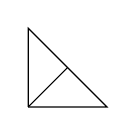
\begin{tikzpicture}
            \draw (0,0) -- (1,0) -- (0, 1) -- (0,0);
            \draw (0,0) -- (0.5, 0.5);
        \end{tikzpicture}

        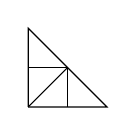
\begin{tikzpicture}
            \draw (0,0) -- (1,0) -- (0, 1) -- (0,0);
            \draw (0,0) -- (0.5, 0.5);
            \draw (0,0.5) -- (0.5, 0.5);
            \draw (0.5,0) -- (0.5, 0.5);
        \end{tikzpicture}
    \end{center}
    
    % \begin{center}
    %     \begin{tikzpicture}
    %         \draw (0,0) -- (1,0);
    %     \end{tikzpicture}
    % \end{center}

    Пусть $\Delta$ - прямоугольний равнобедренный треугольник и $I = [0,1]$. На каждом шаге будем разбивать треугольник и отрезок. На n-ом шаге будет будем иметь $2^n$ треугольников и отрезок, разбитый на столько же частей. Будем занумеровывать треугольники и части отрезка двоичным кодом.
    
    Будем иметь следующую нумерацию: $\Delta_{i_1 \ldots i_n}$ и $I_{i_1 \ldots i_n}$. Определим соседние элементы как элементы, у которых есть общая сторона(для разбиения треугольников), общая точка(для разбиения отрезка).
    Так же мы имеем цепочку вложенных отрезков(треугльников).
    \[
        I_{i_1} \supset I_{i_1 i_2} \supset I_{i_1 i_2 i_3} \supset \ldots
    \]
    \[
        \Delta_{i_1} \supset \Delta_{i_1 i_2} \supset \Delta_{i_1 i_2 i_3} \supset \ldots
    \]
    Эти цепочки имеют строго убывающий размер.

    Из элементарных геометрических соображений можно получить значение диаметров этих множеств.
    \[
        diam(I_{i_1 i_2 \ldots i_n}) = \br{\frac{1}{2}}^n
    \]
    \[
        diam(\Delta_{i_1 \ldots i_n}) = \frac{1}{(\sqrt{2})^{n - 1}}
    \]

    Очевидно, что все эти подмножества компакты(т.к. замкнутые и ограниченные подмножества полного метрического пространства).

    \begin{nota_bene}
        Рассказ про игру.
    \end{nota_bene}

    Определим отображение $f: I \rightarrow I \times I$.

    1) Рассмотрим $t \in I = [0, 1]$. Для $t$ будет существовать последовательность убывающий отрезков
    \[
        t \in I_{i_1} \supset I_{i_1 i_2} \supset I_{i_1 i_2 i_3} \supset \ldots
    \]
    Т.к. $t$ может лежать на границе отрезков, то последовательность определенна неоднозначно.
    Возьмем последовательность треугольников с теми же индексами. Это будет последовательность вложенные компактов, причем дивметр этого множества стремится к $0$. Т.о. пересечение этих треугольников будет состоять из одной точки, эту единственную точку обозначим за $f(t)$.

    % todo: доопределить P_n(t)
    У этого рассуждения есть недостаток, $t$ может принадлежать двум множествам $I_{i_1 \ldots i_n}$ и $I_{j_1 \ldots j_n}$. но в этом случае может объядинить эти два множества и получить $J_{i_1 \ldots i_n}$, также определим множество $P_n(t) = \cbr{}$. (если $t$ - хорошее, то $P_n(t) = \Delta_{i_1 \ldots i_n}$, если $t$ - плохое, то $P_n(t) = $ объединению двух соседних треугольников). 

    Получим еще одну последовательность компактов:
    \[
        P_1(t) \supset P_2(t) \supset \ldots
    \]

    \begin{statement}
        \[
            diam P_n \leq \frac{1}{(\sqrt{2}^{n - 2})}
        \]
    \end{statement}
    Опять получили последовательность вложенных компактов..


    Докажем, что $f$ - сюръективно. 
    Рассмотрим точку $x_0$ из треугольника. Точка будет лежать в определнном последовательность "разрезанных" треугольников. Рассмотрим последовательность подотрезков с теми же индексами, у этой последовательности будет одной общая точка. Остается доказать, что это точка - прообраз точки $x_0$. Это верно, т.к. иначе бы образы этих точек лежали бы в разных треугольниках.

    Докажем, что $f$ - непрерывно. - Очевидно.
\end{proof}

\begin{definition}
    $f_n : X \rightarrow \R$ - последовательность функций.

    $f_n \rightrightarrows 1$, если для каждого $\varepsilon > 0$ сущесвтует $N \in \N$ такое что для каждого $m \geq N$ для каждого $x \in X$ выполняется $|f_n(x) - f(x)| < \varepsilon$
\end{definition}

\begin{theorem}
    Предел равномерно сходящийся функций непрерывен.
\end{theorem}
